\section*{Problems}

\begin{enumerate}[itemsep=6pt]
%  \item Two ice skaters, a large man and a small woman, are initially at
%  rest and holding each other's hands. They push away horizontally. Afterwards,
%  which of the following statements is true?
%  \begin{choices}
%    \choice They have equal and opposite kinetic energies.
%    \choice The have equal and opposite momenta.
%    \choice The large man applies a greater force to the small woman.
%    \choice The small woman applies a greater force to the large man.
%    \choice They recoil with equal and opposite velocities.
%  \end{choices}
%
%  \item Which of the following has the greatest magnitude of momentum?
%  \begin{choices}
%    \choice A \SI{500}{\kilo\gram} car moving at \SI{40}{\metre\per\second}
%    \choice A \SI{30000}{\kilo\gram} dump truck at rest
%    \choice A \SI{1000}{\kilo\gram} SUV moving at \SI{25}{\metre\per\second}
%    \choice A proton moving at \SI{90}{\percent} of the speed of light
%    \choice A \SI{90000000}{\kilo\gram} aircraft carrier moving at
%    \SI2{\centi\metre\per\second}
%  \end{choices}
%
%  \item The momentum change of an object exactly equals which of the
%  following?
%  \begin{choices}
%    \choice The net force acting on the object
%    \choice The velocity change of the object
%    \choice The product of net force and the time the net force acts
%    \choice The product of net force and the change in velocity
%    \choice The ratio of net force and mass
%  \end{choices}
%  
%%  \item In a particular crash safety test, engineers study what happens
%%  when cars hit solid walls. Which of the following observations best indicates
%%  that the \emph{least} amount of force is exerted on the car?
%%  \begin{choices}
%%    \choice The car hits the wall and bounces back.
%%    \choice The car crushes during the collision.
%%    \choice The crash dummy flies through the windshield.
%%    \choice The front seat airbags are deployed.
%%    %\choice The wall crumbles upon collision.
%%  \end{choices}
%  
%  \item A \SI{1000}{\kilo\gram} railroad car is rolling without friction on
%  a horizontal track at a speed of \SI3{\metre\per\second}. Sand is poured into
%  the open top of the car for a time of \SI5\second. The speed of the car after
%  \SI5{\second} is \SI1{\metre\per\second}. The mass of the sand added to the
%  car at the end of \SI5{\second} is
%  \begin{choices}
%    \choice\SI{500}{\kilo\gram}
%    \choice\SI{100}{\kilo\gram}
%    \choice\SI{2000}{\kilo\gram}
%    \choice\SI{3000}{\kilo\gram}
%    \choice\SI{3500}{\kilo\gram}
%  \end{choices}
%  
%  \item A \SI4{\kilo\gram} cart moving to the right with \SI{18}{\joule}
%  of kinetic energy has a head-on collision with a \SI2{\kilo\gram} cart moving
%  to the left with \SI1{\joule} of kinetic energy. After the collision, the
%  \SI4{\kilo\gram} cart continues moving to the right, but its kinetic energy
%  decreases to \SI2\joule. The \SI2{\kilo\gram} cart is driven to the right,
%  but its kinetic energy increases to \SI9\joule. Which of the following is
%  true about this collision?
%  \begin{choices}
%    \choice This is an inelastic collision that demonstrates momentum
%    conservation.
%    \choice This is an elastic collision that demonstrates momentum
%    conservation.
%    \choice This is an inelastic collision where momentum is not conserved.
%    \choice This is an elastic collision where momentum is not conserved.
%    \choice This is a perfectly inelastic collision in which energy is
%    conserved.
%  \end{choices}  
%  \newpage
  
\item In a game of egg-toss, you and a partner are throwing an egg back and
  forth trying not to break it. Given your knowledge of momentum, give two
  hints to your partner to keep the force of impact on the egg as low as
  possible? Clearly explain your answer.

%%  \item Does the situation depicted below defy the law of conservation of
%%  momentum? Explain.\\
%%  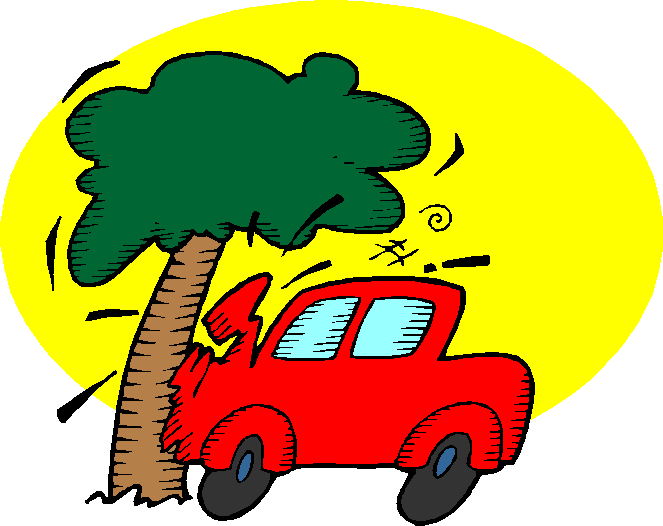
\includegraphics[width=1.75in]{../graphics/a2Homework-img1}
%%  \vspace{\stretch1}
  
\item In a crash test, a car strikes a wall with an average force of 
  \SI{1.23e7}{\newton} [S] over an interval of \SI{21.0}{\milli\second}.
  Calculate the impulse the car exerts on the wall.
  
\item In a crash test similar to the one described in the last problem, another
  car, with the same mass and velocity as the first car, experiences an impulse
  identical to the value you calculated in the last problem. However, the
  second car is designed to crumple more slowly than the first. As a result,
  the duration of the crash is \SI{57.1}{\milli\second}. Determine the average
  force the wall exerted on the second car.
  
\item A \SI{1385}{\kilo\gram} cannon containing a \SI{58.5}{\kilo\gram} cannon
  ball is on wheels. The cannon fires the cannon ball, giving it a velocity of
  \SI{49.8}{\metre\per\second} [N]. What is the initial velocity of the cannon
  the instant after it fires the cannon ball?
 
\item Two amusement park bumper cars are heading directly towards each other.
  The combined mass of car A plus driver is \SI{375}{\kilo\gram} and it is
  moving with a velocity of $+$\SI{1.8}{\metre\per\second}. The combined mass
  of car B plus driver is \SI{422}{\kilo\gram} and it is moving with a velocity
  of \SI{-1.4}{\metre\per\second}. When they collide, they become stuck
  together and continue moving along the same straight line. What is their
  velocity immediately after they collide?

%  \item An \SI{80}{\kilo\gram} astronaut has become detached from the
%  safety line connecting her to the International Space Station. She is
%  \SI{200}{\metre} from the station, and at rest relative to it. She only has
%  4.0 minutes of air remaining. To get herself back, she tosses a
%  \SI{10}{\kilo\gram} tool kit away from the station at
%  \SI{8.0}{\metre\per\second}. Will she make it back in time?
%  \vspace{\stretch1}
%  \newpage
%  
%  \item A \SI{2.0}{\kilo\gram} box is initially moving at
%  $+$\SI{3.0}{\metre\per\second} and is pushed along a horizontal, frictionless
%  surface with a net force $F$ that varies with time according to the following
%  graph:
%  \begin{center}
%    \begin{tikzpicture}[yscale=.14]
%      \foreach\x in {1,...,7} \draw(\x,1)--(\x,-1) node[below]{$\x$};
%      \foreach\y in {-10,-5,...,20}{
%        \draw[thin,gray!50] (7.5,\y)--(-.1,\y) node[left,black]{$\y$};
%      }
%      \draw[axes] (0,0)--(7.5,0) node[right]{$t$ (s)};
%      \draw[axes] (0,-13)--(0,25) node[above]{$F$ (N)};
%      \draw[ultra thick] (0,20)--(1,20)--(3,0)--(4,0)--(5,-10)--(7,-10);
%    \end{tikzpicture}
%  \end{center}
%  \begin{enumerate}[itemsep=3pt]
%    \item In the table below, indicate the momentum change of the box during
%    each second of elapsed time.
%    \begin{center}
%      {\large
%        \begin{tabular}{c|c}
%          Time (s) & Impulse (\si{\newton\second}) \\\hline
%          $0-1$ &\\
%          $1-2$ &\\
%          $2-3$ &\\
%          $3-4$ &\\
%        \end{tabular}
%        \hspace{.7in}
%         \begin{tabular}{c|c}
%          Time (s) & Impulse (\si{\newton\second}) \\\hline
%          $4-5$ &\\
%          $5-6$ &\\
%          $6-7$ &\\
%           & 
%        \end{tabular}
%      }
%    \end{center}
%
%    \item Plot the velocity vs.\ time graph for this motion in the space below.
%    Label all relevant quantities on the $x$ and $y$ axis.
%    \begin{center}
%      \begin{tikzpicture}[scale=.8]
%        \draw[gray!40] grid (7,8);
%        \draw[axes] (0,0)--(0,8.5) node[above]{$v$ (\si{\metre\per\second})};
%        \draw[axes] (0,0)--(7.5,0) node[right]{$t$ (\si\second)};
%      \end{tikzpicture}
%    \end{center}
%    \item At $t=\SI{7.0}\second$, the box collides with a wall and bounces
%    backwards at \SI{6.0}{\metre\per\second}. Given that the box is in contact
%    with the wall for \SI{.20}\second, calculate the average force that the
%    wall exerts on the box.
%
%  \end{enumerate}
%  \newpage
%  
%%  \item A billiard ball of mass \SI{0.155}{\kilo\gram} (``cue ball'') moves
%%  with a velocity of \SI{12.5}{\metre\per\second} towards a stationary billiard
%%  ball (``eight ball'') of identical mass and strikes it with a glancing blow.
%%  The cue ball moves off at an angle of \ang{29.7} clockwise from its original
%%  direction, with a speed of \SI{9.56}{\metre\per\second}.
%%  \begin{enumerate}[itemsep=3pt]
%%    \item What is the velocity of the eight ball?
%%    \item Determine whether the collision was elastic.
%%  \end{enumerate}
  
\item A \SI{1875}{\kilo\gram} car is travelling along a country road when the
  driver sees a deer dart out onto the road. The driver slams on the brakes
  and manages to stop before hitting the deer. The driver of a second car (mass
  \SI{2135}{\kilo\gram}) is driving too close. When the driver realizes that
  the car ahead has stopped, he hits the brakes but is unable to stop. The two
  cars lock together and skid another \SI{4.58}{\metre} along a straight line
  before coming to a stop. If the coefficient of friction between concrete and
  rubber is 0.750, what is the speed of the second car when it hits the stopped
  car?

\item While playing a game of billiards, your \SI{.17}{\kilo\gram} cue ball,
  travelling at \SI{1.9}{\metre\per\second}, glances off a stationary
  \SI{.16}{\kilo\gram} ``eight ball'' so that the eight ball moves off at
  \SI{1.3}{\metre\per\second} at an angle of \ang{32} clockwise from the cue
  ball's original path.
  \begin{enumerate}[itemsep=3pt]
  \item What is the final velocity (both magnitude and direction) of the cue
    ball?
  \item Calculate the total kinetic energy before and after the collision. Is
    the collision elastic?
  \end{enumerate}

%  \item Two blocks are free to slide along the frictionless wooden track
%  shown below. The block of mass $m_1=\SI{4.98}{\kilo\gram}$ is released from
%  the position shown, at height $h=\SI{5.00}\metre$ above the flat part of the
%  track. Protruding from its front end is the north pole of a strong magnet,
%  which repels the north pole of an identical magnet embedded in the back end
%  of the block of mass $m_2=\SI{9.40}{\kilo\gram}$, initially at rest. The two
%  blocks never touch.
%  \begin{center}
%    \begin{tikzpicture}
%      \draw[thick,fill=brown!50] (0,0)--(0,4)--(1,4)--(1,3.5) to[out=270,in=180]
%      (5,.5)--(12,.5)--(12,0)--(0,0);
%      \draw[thick,dashed] (.2,.5)--(5,.5);
%      \draw[thick,dashed] (.2,3.5)--(1,3.5);
%      \draw[<->,thick] (.5,.5)--(.5,3.5) node[midway,fill=brown!50]{$h$};
%      \draw[mass] (5.2,.5) rectangle (5.8,.9) node[right=-1]{$m_2$};
%      \draw[mass] (1,4) rectangle (1.4,3.5)
%      node[right=0]{$m_1$};
%    \end{tikzpicture}
%  \end{center}
%  Calculate:
%  \begin{enumerate}[itemsep=3pt]
%    \item The speed of $m_1$ just before the collision
%    \item The velocities of $m_1$ and $m_2$ after the elastic collision
%    \item The maximum height to which $m_1$ rises after the elastic collision
%  \end{enumerate}
\end{enumerate}

